\subsection{Sufficiency of the predicted seeds inside Kira}
\label{sec:seed-kira-sufficiency}
To determine whether the predicted seeds supply enough equations,
we use Kira~3.1 to test whether each target belongs to the span of
its specified masters modulo the available identities. This means
that the target can be written as a linear combination of those
masters after using the selected equations. We retain the frozen
model, reserved families and threshold of one half from
Eq.~\eqref{eq:seed-predicted-set}.

Let $\mathcal E_{\boldsymbol\sigma}$ contain the stored IBP identities
from seed $\boldsymbol\sigma$, and let $\mathcal B$ contain the
background identities, including partial fractions and symmetries.
A supplied seed set $\mathcal S$ provides the equations
\begin{equation}
 \mathcal A(\mathcal S)
 =\mathcal B\cup
       \bigcup_{\boldsymbol\sigma\in\mathcal S}
                       \mathcal E_{\boldsymbol\sigma}.
 \label{eq:kira-selected-relations}
\end{equation}
Every selected seed contributes all its stored IBP identities.
The reference seed labels, construction paths and master coefficients
supply no equations to this test.

The sufficiency condition follows from linear algebra over the field
$\mathbb K=\mathbb Q(\boldsymbol x,d)$ of rational functions in the
kinematic parameters $\boldsymbol x$ and dimension $d$.
Let $V$ be the vector space with one formal basis vector for each
integral in the supplied system, let $v_{\mathcal T}$ be the coefficient
vector of the target, and let $\mathcal R(\mathcal S)$ be the row space
of the equations in $\mathcal A(\mathcal S)$. Also let
$V_M$ be the span of the basis vectors for the specified
masters. Then
\begin{equation}
 \begin{aligned}
 \mathcal T=\sum_m r_{\mathcal Tm} M_m
 \quad\hbox{using }\mathcal A(\mathcal S)
 &\quad\Longleftrightarrow\quad
 v_{\mathcal T}\in\mathcal R(\mathcal S)+V_M,\\
 &\quad\Longleftrightarrow\quad
 [v_{\mathcal T}]=0
 \quad\hbox{in }V/(\mathcal R(\mathcal S)+V_M).
 \end{aligned}
 \label{eq:kira-master-span}
\end{equation}
Here $M_m$ is a specified master, $r_{\mathcal Tm}\in\mathbb K$ is its reduction
coefficient, and square brackets denote the equivalence class after
removing combinations of available equations and master vectors.
This condition tests whether such coefficients exist without
requiring their full symbolic reconstruction.
Sufficiency applies to the supplied target expression and permits
exact cancellation among its terms.

We implement the condition through Kira's user-defined-equation
interface, which accepts homogeneous linear systems with rational
coefficients and uses Fermat for symbolic operations
\cite{Kira12,Kira3}. Each target has an auxiliary variable
$Z_{\mathcal T}$ and the input equation
\begin{equation}
 Z_{\mathcal T}
 -\sum_{j=1}^{n_T}c_j(\boldsymbol x,d)
                         I_{\boldsymbol a^{(j)}}=0.
 \label{eq:kira-target-definition}
\end{equation}
All terms in this equation come from the public target expression
in Eq.~\eqref{eq:seed-model-input}. We add one unit row for each
specified master vector. These rows impose $M_m=0$ in the formal
quotient used for the test, where every possible master combination
represents zero. They do not change the physical values of the
master integrals.

Kira reduces $Z_{\mathcal T}$ exactly in this system. A zero remainder
establishes the condition in Eq.~\eqref{eq:kira-master-span}, and a
nonzero remainder shows that the supplied equations leave an
independent contribution outside the specified master span.
The conclusion applies to rational functions at generic parameter
values where their denominators are defined. A successful program
exit alone does not establish sufficiency.

Different seed sets use separate copies of every integral variable
so that they cannot share equations. Targets with the same selected
set can share a system within one family. We retain every equation
in a component connected to the target terms and remove only
disconnected components. For each target we test its predicted set,
the full candidate set $\mathcal C$, and the empty seed set.
The full set checks the available fallback, while the empty set
measures reduction through the target definition, master basis and
background identities alone.

We independently reconstruct the selected row spaces from the
original identities at each of the three stored finite-field
samples. At each sample, sparse elimination checks membership after
removing master columns and must agree with Kira's symbolic decision.
Each nonzero symbolic remainder also has a regular sample with a
nonzero value, which provides an exact witness that its coefficient
does not vanish identically. The sample coordinates enter these
checks after the symbolic calculation; reference master coefficients
remain outside the full sufficiency test. For two pilot
families, 765 target-and-seed-set comparisons also agree with
reductions that retain the masters and compare their explicit
rational coefficients.

\subsection{Sufficiency results and the role of additional seeds}
The test includes all 690,382 reserved targets from 5,137
families. The predicted sets supply enough equations for 652,517
targets (94.515\%), while 37,865 (5.485\%)
have a nonzero remainder outside the master span.
The full candidate pool is sufficient for 690,382 targets
(100.000\%), and background identities alone suffice for
26,915 (3.899\%).
Within the coupled-vacuum subset, the predicted sets suffice for
595,919 of 618,240
targets (96.390\%).
Within the one-loop box subset, they suffice for
56,294 of 71,184
targets (79.082\%).
For the other one-loop samples, the predicted sets suffice for
89 of 380 bubble targets (23.421\%), 152 of 431 triangle targets (35.267\%), 60 of 144 propagator targets (41.667\%), and 3 of 3 tadpole targets (100.000\%). The overall fraction therefore depends on the
mixture of tested family domains.
All symbolic membership decisions agree with the independent
row-space checks at the three stored samples.
All requested targets have a recorded outcome, and the final
evaluation has no unresolved solver or export errors
\cite{KiraSeedSufficiencyData}.

\begin{figure}[htbp]
 \centering
 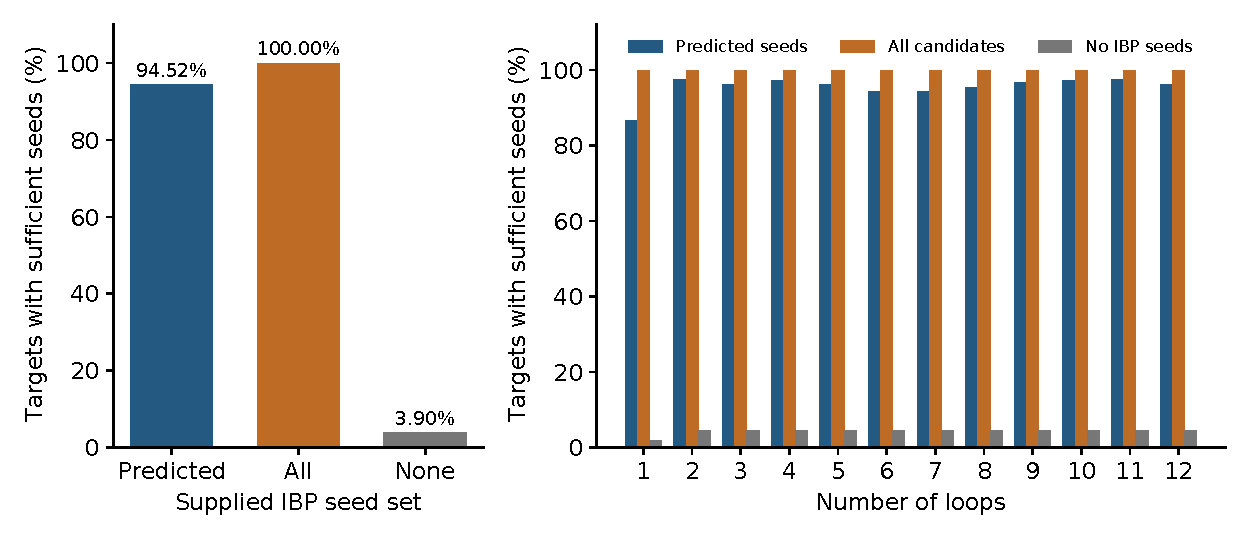
\includegraphics[width=\linewidth]{figures/kira_seed_sufficiency.pdf}
 \caption{Targets that belong to the specified master span after
 using the supplied identities, shown for predicted seeds, all
 candidate seeds and no IBP seeds. Each loop-order fraction uses every reserved target at that
 order. All three policies retain the same background identities.}
 \label{fig:kira-seed-sufficiency}
\end{figure}

Of the targets with sufficient predicted sets, 70,302
use a seed set different from the recorded reference set.
This comparison shows that a model can supply enough equations
through an alternative selection, so reference-set agreement and
algebraic sufficiency measure different properties.
The model selects 3.439 seeds per target on
average. Across all target--candidate pairs, it selects
3.102\% of the supplied candidates.
This fraction describes selection within the bounded pools; it
does not measure a runtime improvement over Kira's usual strategies.

\begin{figure}[htbp]
 \centering
 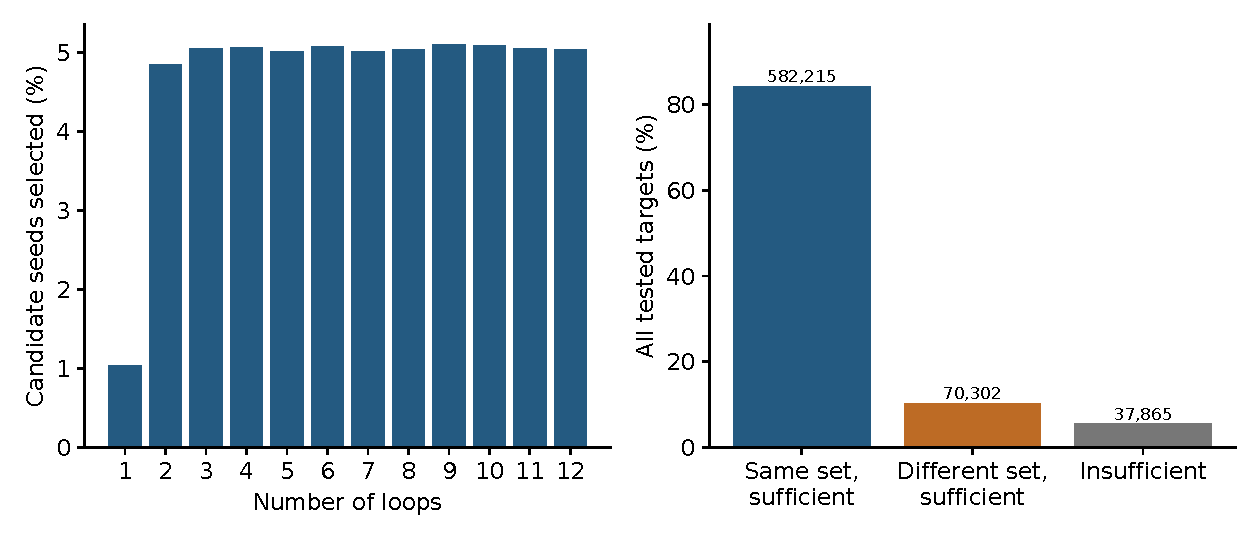
\includegraphics[width=\linewidth]{figures/kira_seed_sets.pdf}
 \caption{The selected fraction of candidate seeds at each loop
 order, and the relation between reference-set agreement and seed sufficiency
 in Kira. Numbers above the bars are target counts.
 Different sufficient sets account for the difference between the
 two tests.}
 \label{fig:kira-seed-sets}
\end{figure}

The all-candidate control supplies a direct check of the fallback
within the stored equation domain. A predicted set that leaves
extra integrals requires further equations before we accept its
reduction. We solve the full-pool control independently, which checks whether
adding all candidates would supply a sufficient fallback. This test
does not identify the smallest necessary addition or measure reuse
of a preceding elimination.
Its conclusions concern rational functions at generic parameter
values, where the denominators in the reduction are defined.

These results establish algebraic sufficiency rates inside Kira
for the stored identities. The user-defined interface is needed
for the present family representation, including the dependent
massive denominators of the higher-loop vacuum families.
An insufficient outcome refers to the stored identities for the
selected seeds. Additional valid IBP operators at the same seeds can
enlarge that pool. Section~\ref{sec:cost-comparison} separately compares native Kira
seeding through learned sector bounds with the stated native baselines. The grouped
execution also shares work among targets with identical selected
sets, so its elapsed times do not provide an end-to-end solver
speedup measurement. The next section addresses the separate
learned choice of an allowed elimination step.
